%% =============================================================================
%%  fig_filter.tex -- the snoop filter's internal mechanism, standalone.
%%
%%  Build:  pdflatex fig_filter.tex   ->  fig_filter.pdf
%%
%%  Redrawn 2026-09-13 in the terminology of the paper's Section V, so that
%%  every block and signal here is defined in the text:
%%    update port from each DCU: "tag + valid update" (the signals that write
%%        its Status-RAM and Tag-RAM), and "fill in flight + address"
%%    the INV REQ selected by the INV REQ arbiter: issued by PE i, address of w
%%        = set index . tag
%%    per (PE, way): Tag-RAM mirror (LUTRAM, read at the set index of w),
%%        valid bit (flip-flop), compare "stored tag = tag of w AND valid"
%%    per PE: OR over the two ways -> "holds the line"; fill compare ->
%%        "is fetching the line"; OR -> "holds or is fetching"
%%    exclude the requesting PE i -> sharer set S(w);  S(w) = empty -> suppress
%%        the broadcast, else broadcast and grant by condition (1)
%%
%%  Routing rule, so that no two lines cross: the "address of w" is one bus
%%  that threads left to right through every block that reads it (Tag-RAM
%%  mirror, valid bit, fill compare); those blocks take their DCU inputs from
%%  above, the compare block hangs below the bus and takes "tag of w" from a
%%  tap (junction dot), and all results flow downwards in their own columns.
%%  PE 0 is drawn in full; PE 1-3 are identical and drawn collapsed.
%% =============================================================================
\documentclass[border=3pt]{standalone}
\usepackage{tikz}
\usepackage{times}
\usepackage{amssymb}
\usetikzlibrary{arrows.meta,calc}

\begin{document}
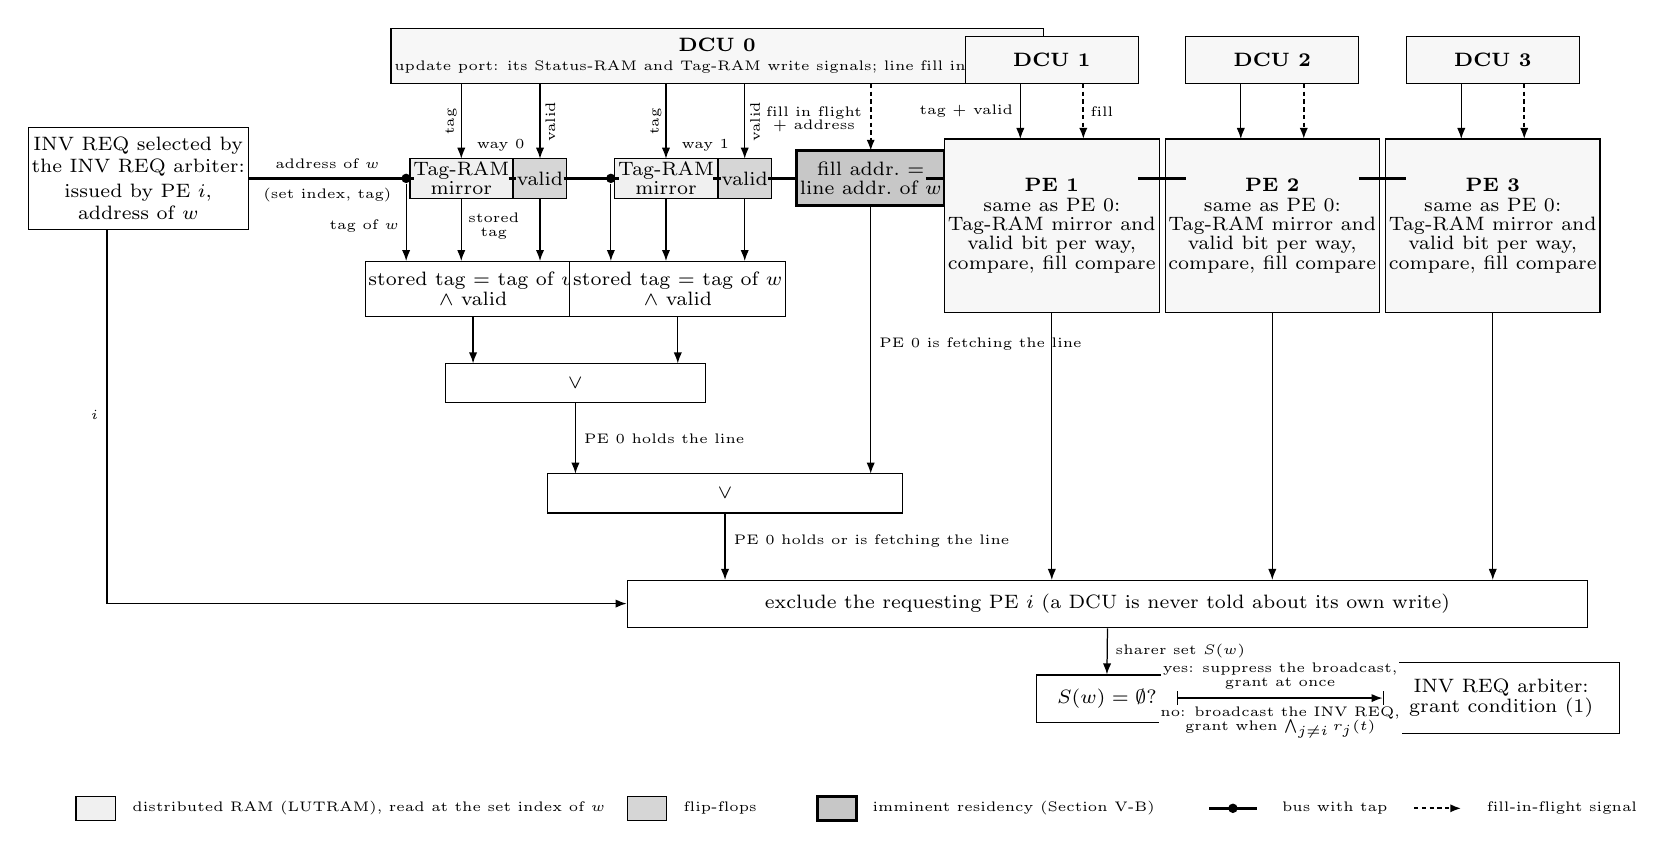
\begin{tikzpicture}[
  x=1mm, y=1mm, font=\scriptsize,
  box/.style  ={draw,rectangle,align=center,inner sep=1.2pt},
  ram/.style  ={box,fill=black!6},
  ff/.style   ={box,fill=black!16},
  op/.style   ={box,fill=white},
  pe/.style   ={box,fill=black!3},
  src/.style  ={box,fill=white},
  new/.style  ={box,fill=black!22,line width=1.1pt},
  ln/.style   ={draw,-{Latex[length=1.4mm]},line width=0.45pt},
  wire/.style ={draw,line width=0.45pt},
  bus/.style  ={draw,line width=1.1pt},
  mir/.style  ={draw,-{Latex[length=1.4mm]},dashed,dash pattern=on 1.6pt off 1.2pt,line width=0.7pt},
  dot/.style  ={circle,fill=black,inner sep=0,minimum size=1.2mm},
  lab/.style  ={font=\tiny,inner sep=0.7pt,fill=white,align=center},
  labr/.style ={font=\tiny,inner sep=0.4pt,rotate=90,anchor=center},
]

% ----------------------------------------------------------- the request
\node[src,minimum width=24mm,minimum height=13mm,anchor=east] (srcb) at (-18, 0)
  {INV REQ selected by\\the INV REQ arbiter:\\[1pt]
   issued by PE $i$,\\address of $w$};
% the "address of w" bus starts here and threads through every block that reads it
\draw[bus] (-18, 0) -- (2, 0);
\node[lab,anchor=south] at (-8, 0.9) {address of $w$};
\node[lab,anchor=north] at (-8, -0.9) {(set index, tag)};
% the requester's index goes straight down to the exclusion row
\draw[ln] (-36, -6.5) -- (-36, -54) -- (30, -54);
\node[lab,anchor=east] at (-36.8, -30) {$i$};

% ----------------------------------------------------------- PE 0 in full
\node[pe,minimum width=68mm,minimum height=7mm,anchor=south west] (dcu0) at (0, 12)
  {\textbf{DCU 0}\\[-1pt] {\tiny update port: its Status-RAM and Tag-RAM write signals; line fill in progress}};

% two ways, centres c = 12 and 38
\foreach \k/\c in {0/12, 1/38} {
  % on the bus: tap for "tag of w", then the Tag-RAM mirror, then the valid bit
  \node[dot] (tp\k) at (\c-10, 0) {};
  \node[ram,minimum width=12mm,minimum height=5mm] (tr\k) at (\c-3, 0)
    {Tag-RAM\\[-1pt]mirror};
  \node[ff,minimum width=6mm,minimum height=5mm] (vb\k) at (\c+7, 0) {valid};
  \draw[bus] (\c-11, 0) -- (\c-9, 0);
  \draw[bus] (\c+3, 0) -- (\c+4, 0);
  \draw[bus] (\c+10, 0) -- (\c+16, 0);
  % update port from DCU 0, straight down into both
  \draw[ln] (\c-3, 12) -- (\c-3, 2.5);
  \draw[ln] (\c+7, 12) -- (\c+7, 2.5);
  \node[labr] at (\c-4.3, 7.2) {tag};
  \node[labr] at (\c+8.3, 7.2) {valid};
  \node[lab] at (\c+2, 4.2) {way \k};
  % compare block below, fed by the tap, the stored tag and the valid bit
  \node[op,minimum width=20mm,minimum height=7mm] (cp\k) at (\c-1.5, -14)
    {stored tag $=$ tag of $w$\\[-1pt] $\wedge$ valid};
  \draw[ln] (tp\k) -- (\c-10, -10.5);
  \draw[ln] (tr\k.south) -- (\c-3, -10.5);
  \draw[ln] (vb\k.south) -- (\c+7, -10.5);
  % result of this way goes down to the OR
  \draw[ln] (cp\k.south) -- (\c-1.5, -23.5);
}
\node[lab,anchor=east] at (1.4, -6) {tag of $w$};
\node[lab,anchor=west] at (9.6, -6) {stored\\[-1pt]tag};

% fill compare, also on the bus, also fed from DCU 0
\node[new,minimum width=14mm,minimum height=7mm] (fc0) at (61, 0)
  {fill addr.\ $=$\\[-1pt] line addr.\ of $w$};
\draw[mir] (61, 12) -- (61, 3.5);
\node[lab,anchor=east] at (60.2, 7.5) {fill in flight\\[-1pt]+ address};
\draw[bus] (68, 0) -- (73, 0);
\draw[ln] (fc0.south) -- (61, -37.5);
\node[lab,anchor=west] at (61.8, -21) {PE 0 is fetching the line};

% OR over the two ways, then OR with the fill term
\node[op,minimum width=33mm,minimum height=5mm] (or0) at (23.5, -26) {$\vee$};
\draw[ln] (or0.south) -- (23.5, -37.5);
\node[lab,anchor=west] at (24.3, -33) {PE 0 holds the line};
\node[op,minimum width=45mm,minimum height=5mm] (or0b) at (42.5, -40) {$\vee$};
\draw[ln] (or0b.south) -- (42.5, -51);
\node[lab,anchor=west] at (43.3, -46) {PE 0 holds or is fetching the line};

% ----------------------------------------------------------- PE 1..3 collapsed
\foreach \j/\x in {1/84, 2/112, 3/140} {
  \node[pe,minimum width=22mm,minimum height=6mm,anchor=south] (dcu\j) at (\x, 12)
    {\textbf{DCU \j}};
  \node[pe,minimum width=22mm,minimum height=22mm] (blk\j) at (\x, -6)
    {\textbf{PE \j}\\[-1pt] same as PE 0:\\[-1pt] Tag-RAM mirror and\\[-1pt]
     valid bit per way,\\[-1pt] compare, fill compare};
  \draw[ln]  (\x-4, 12) -- (\x-4, 5);
  \draw[mir] (\x+4, 12) -- (\x+4, 5);
  \draw[ln]  (blk\j.south) -- (\x, -51);
}
\draw[bus] (95, 0) -- (101, 0);
\draw[bus] (123, 0) -- (129, 0);
\node[lab,anchor=east] at (79.4, 8.5) {tag + valid};
\node[lab,anchor=west] at (88.6, 8.5) {fill};

% ----------------------------------------------------------- sharer set
\node[op,minimum width=122mm,minimum height=6mm,anchor=north west] (mask) at (30, -51)
  {exclude the requesting PE $i$ (a DCU is never told about its own write)};
\draw[ln] (mask.south) -- (91, -63);
\node[lab,anchor=west] at (91.8, -60) {sharer set $S(w)$};

\node[op,minimum width=18mm,minimum height=6mm,anchor=north] (empty) at (91, -63) {$S(w) = \emptyset$?};
\node[op,minimum width=30mm,minimum height=9mm,anchor=west] (arb) at (126, -66)
  {INV REQ arbiter:\\[-1pt] grant condition (1)};
\draw[ln] (100, -66) -- (126, -66);
\node[lab,anchor=south] at (113, -65.2) {yes: suppress the broadcast,\\[-1pt] grant at once};
\node[lab,anchor=north] at (113, -66.8) {no: broadcast the INV REQ,\\[-1pt] grant when $\bigwedge_{j \ne i} r_j(t)$};

% ----------------------------------------------------------- legend
\node[ram,minimum width=5mm,minimum height=3mm,inner sep=0,anchor=west] at (-40, -80) {};
\node[font=\tiny,anchor=west] at (-34, -80) {distributed RAM (LUTRAM), read at the set index of $w$};
\node[ff,minimum width=5mm,minimum height=3mm,inner sep=0,anchor=west] at (30, -80) {};
\node[font=\tiny,anchor=west] at (36, -80) {flip-flops};
\node[new,minimum width=5mm,minimum height=3mm,inner sep=0,anchor=west] at (54, -80) {};
\node[font=\tiny,anchor=west] at (60, -80) {imminent residency (Section V-B)};
\draw[bus] (104, -80) -- (110, -80); \node[dot] at (107, -80) {};
\node[font=\tiny,anchor=west] at (112, -80) {bus with tap};
\draw[mir] (130, -80) -- (136, -80);
\node[font=\tiny,anchor=west] at (138, -80) {fill-in-flight signal};

\end{tikzpicture}
\end{document}
